% Options for packages loaded elsewhere
\PassOptionsToPackage{unicode}{hyperref}
\PassOptionsToPackage{hyphens}{url}
%
\documentclass[
  english,
  doc,floatsintext]{apa6}

\usepackage{graphicx}
\makeatletter
\def\maxwidth{\ifdim\Gin@nat@width>\linewidth\linewidth\else\Gin@nat@width\fi}
\def\maxheight{\ifdim\Gin@nat@height>\textheight\textheight\else\Gin@nat@height\fi}
\makeatother
% Scale images if necessary, so that they will not overflow the page
% margins by default, and it is still possible to overwrite the defaults
% using explicit options in \includegraphics[width, height, ...]{}
\setkeys{Gin}{width=\maxwidth,height=\maxheight,keepaspectratio}
% Set default figure placement to htbp
\makeatletter
\def\fps@figure{htbp}
\makeatother
\setlength{\emergencystretch}{3em} % prevent overfull lines
\providecommand{\tightlist}{%
  \setlength{\itemsep}{0pt}\setlength{\parskip}{0pt}}
\setcounter{secnumdepth}{5}
% Make \paragraph and \subparagraph free-standing
\ifx\paragraph\undefined\else
  \let\oldparagraph\paragraph
  \renewcommand{\paragraph}[1]{\oldparagraph{#1}\mbox{}}
\fi
\ifx\subparagraph\undefined\else
  \let\oldsubparagraph\subparagraph
  \renewcommand{\subparagraph}[1]{\oldsubparagraph{#1}\mbox{}}
\fi

%\usepackage[utf8x]{inputenc}
\usepackage{amsmath}
\usepackage{amsthm}
\usepackage{graphicx}
\usepackage[colorinlistoftodos]{todonotes}
\usepackage[singlespacing]{setspace}

\let\B\relax 

\let\T\relax

\usepackage{gb4e}
\exewidth{(\thexnumi)} %ex number no indent setting
\let\eachwordone=\textit %first line italic
\noautomath

\usepackage[linguistics,edges]{forest} 
\forestset{
ned/.style={%
    for tree={calign=fixed edge angles},
    delay={%
      where content={}{%
        shape=coordinate,
        for nodewalk={%
          Nodewalk={%
            on invalid=fake,
          }{%
            parent,
          }{%
            for children={anchor=north},
          }
        }{},
      }{},
    },
},
fned/.style={
        delay={where content={}{shape=coordinate,
              for siblings={anchor=north}}{}},
		for tree={s sep=4mm}},
}


\usepackage{leipzig}
\makeglossaries


\usepackage{hyperref}
\hypersetup{colorlinks = true, linkcolor = blue, citecolor = blue, urlcolor = blue}
\usepackage{multicol}
% Manuscript styling
\usepackage{upgreek}
\captionsetup{font=singlespacing,justification=justified}

% Table formatting
\usepackage{longtable}
\usepackage{lscape}
% \usepackage[counterclockwise]{rotating}   % Landscape page setup for large tables
\usepackage{multirow}		% Table styling
\usepackage{tabularx}		% Control Column width
\usepackage[flushleft]{threeparttable}	% Allows for three part tables with a specified notes section
\usepackage{threeparttablex}            % Lets threeparttable work with longtable

% Create new environments so endfloat can handle them
% \newenvironment{ltable}
%   {\begin{landscape}\begin{center}\begin{threeparttable}}
%   {\end{threeparttable}\end{center}\end{landscape}}
\newenvironment{lltable}{\begin{landscape}\begin{center}\begin{ThreePartTable}}{\end{ThreePartTable}\end{center}\end{landscape}}

% Enables adjusting longtable caption width to table width
% Solution found at http://golatex.de/longtable-mit-caption-so-breit-wie-die-tabelle-t15767.html
\makeatletter
\newcommand\LastLTentrywidth{1em}
\newlength\longtablewidth
\setlength{\longtablewidth}{1in}
\newcommand{\getlongtablewidth}{\begingroup \ifcsname LT@\roman{LT@tables}\endcsname \global\longtablewidth=0pt \renewcommand{\LT@entry}[2]{\global\advance\longtablewidth by ##2\relax\gdef\LastLTentrywidth{##2}}\@nameuse{LT@\roman{LT@tables}} \fi \endgroup}

% \setlength{\parindent}{0.5in}
% \setlength{\parskip}{0pt plus 0pt minus 0pt}

% \usepackage{etoolbox}
\makeatletter
\patchcmd{\HyOrg@maketitle}
  {\section{\normalfont\normalsize\abstractname}}
  {\section*{\normalfont\normalsize\abstractname}}
  {}{\typeout{Failed to patch abstract.}}
\patchcmd{\HyOrg@maketitle}
  {\section{\protect\normalfont{\@title}}}
  {\section*{\protect\normalfont{\@title}}}
  {}{\typeout{Failed to patch title.}}
\makeatother
\shorttitle{Agreement Attraction in Turkish}
\keywords{keywords\newline\indent Word count: X}
\usepackage{csquotes}
\geometry{left=25mm, right=25mm, top=25mm, bottom=25mm}


\ifxetex
  % Load polyglossia as late as possible: uses bidi with RTL langages (e.g. Hebrew, Arabic)
  \usepackage{polyglossia}
  \setmainlanguage[]{english}
\else
  \usepackage[shorthands=off,main=english]{babel}
\fi
\ifluatex
  \usepackage{selnolig}  % disable illegal ligatures
\fi
\newlength{\cslhangindent}
\setlength{\cslhangindent}{1.5em}
\newenvironment{cslreferences}%
  {\setlength{\parindent}{0pt}%
  \everypar{\setlength{\hangindent}{\cslhangindent}}\ignorespaces}%
  {\par}

\title{Agreement Attraction in Turkish}
\author{Utku Türk\textsuperscript{1}}
\date{}


\authornote{

authornote

Correspondence concerning this article should be addressed to Utku Türk, Postal address. E-mail: \href{mailto:utku.turk@boun.edu.tr}{\nolinkurl{utku.turk@boun.edu.tr}}

}

\affiliation{\vspace{0.5cm}\textsuperscript{1} Boğaziçi University University, Istanbul, Turkey}

\abstract{
We report the results of two speeded acceptability judgment experiments in Turkish. We hypothesized an alternative explanation for agreement attraction effects in Turkish that is based on shallow processing. Our findings contradict our hypothesized form-driven processing strategy and support an account of agreement attraction based on the use of abstract linguistic features, rather than mere form.
}



\begin{document}
\maketitle

\hypertarget{introduction}{%
\section{Introduction}\label{introduction}}

It has been observed that speakers often fail to accurately process grammatical dependencies between the parts of a sentence (Gibson \& Thomas, 1999; Phillips, Wagers, \& Lau, 2011).
For example, ungrammatical center-embedded structures like \emph{The patient who the nurse who the clinic had hired met Jack} are found grammatical by native English speakers.
One such comprehension error is agreement attraction (Nicol, Forster, \& Veres, 1997; Pearlmutter, Garnsey, \& Bock, 1999; Wagers, Lau, \& Phillips, 2009).
Speakers may erroneously find sentences acceptable in which the verb erroneously agrees with a syntactically unrelated noun phrase (\emph{the attractor}) instead of the subject (\emph{the agreement controller}) as in \ref{item:wagers2009}.

\begin{exe}
\ex \label{item:wagers2009} * The key to the cells are rusty from many years of disuse. 
\end{exe}

These effects were found to be robust in a variety of constructions in different languages, e.g.~English , German , Russian, Arabic, Spanish, Armenian, Slovak, Greek, and Turkish (Avetisyan, Lago, \& Vasishth, 2020; Badecker \& Kuminiak, 2007; Lago et al., 2018; Lago, Shalom, Sigman, Lau, \& Phillips, 2015; Paspali \& Marinis, 2020; Reifegerste, Hauer, \& Felser, 2016; Tucker, Idrissi, \& Almeida, 2015) using structures like object relative clauses, subject relative clauses, possessive relative clauses, and genitive-possessive noun phrases (Dillon, Clifton, \& Frazier, 2013; Franck, Colonna, \& Rizzi, 2015; Häussler \& Bader, 2009; Lago et al., 2018, 2015; Parker, Lago, \& Phillips, 2015; Tucker et al., 2015; Wagers et al., 2009). These effects are found both in grammatical marking of the gender and the number (Badecker \& Kuminiak, 2007; Paspali \& Marinis, 2020; Slioussar \& Malko, 2016), and attested with various methods including maze tasks, ERP, eye tracking to name a few (Nicol et al., 1997; Tanner, Nicol, \& Brehm, 2014; Wagers et al., 2009).

One instance of agreement attraction is found in the production processes in which participants were asked to complete sentence fragments (Bock \& Miller, 1991). Participants used the wrong verb more often when the attractor (\emph{cabinets}) were plural, and the agreement controller (\emph{key}) were singular as in \ref{item:bock1991}.

\begin{exe}
\ex The key to the cabinets \ldots 
\label{item:bock1991}
\end{exe}

Agreement attraction is also found in the comprehension studies. In these studies, agreement attraction is found either as a facilitation in reading times or as a effect in the acceptability rates (Wagers et al., 2009).
When reading times are checked, they found that the participants read the ungrammatical sentences with a plural attractor easier then the ungrammatical sentences without a plural attractor.
Similarly, participants found ungrammatical sentences with a plural attractor acceptable more often than that of with a singular attractor.

Some theories (Eberhard, Cutting, \& Bock, 2005; Hammerly, Staub, \& Dillon, 2019) explain this phenomenon through a faulty representation of the number on the head of the agreement controller whereas other theories assume that agreement attraction is due to an error in the access to the number of the agreement controller (Nicenboim, Vasishth, Engelmann, \& Suckow, 2018; Wagers et al., 2009).

Agreement attraction effects can equally well be explained by assuming shallow processing. Recent studies in psychology literature show that in certain environments people may not notice ungrammaticalities in a sentence or may not compute dependencies in a sentence completely (Ferreira, Bailey, \& Ferraro, 2002; Otero \& Kintsch, 1992).

To investigate this possibility, we report two speeded acceptability judgment experiments in this paper. The first one inspects the recent Lago et al. (2018) findings. They found number attraction effects in genitive-possessive constructions such as `\emph{{[}{[}the child's{]} toy{]}}' ({[}{[}\emph{çocuğ-un\textsubscript{Gen}}{]} \emph{oyuncağ-ı\textsubscript{Poss}}{]}). They justify the use of this construction with the findings of Nicol, Barss, and Barker (2016). Since the genitive case is a possible subject marker, the participants can consider genitive marked attractors a candidate for the agreement controller. However, case marking on all subject heads is locally ambiguous the accusative and the possessive. In our experiment 1, we disambiguate the subject head and test whether or not the results were due to the shallow processing of the head subject and sticking with the accusative marked representation under some conditions.

In experiment 2, we test whether or not the agreement attraction effects in Turkish are due to form-driven processing strategy. Instead of processing the whole sentence, participants develop a mental shortcut, matching the form-identical number marking on the attractor and the matrix verb in the Turkish case, specific to the task in hand. We used the verbs of the object relative clauses as an attractor and speculated that if the participants are using the mentioned task-specific strategy, we would see comparable agreement attraction effects.

This paper is organized as \ldots 

\hypertarget{theories-of-agreement-attraction}{%
\section{Theories of agreement attraction}\label{theories-of-agreement-attraction}}

The difference between the theories that explain the agreement attraction phenomenon lies in the assumption regarding the origin of the illusion. Some theories (Bergen \& Gibson, 2012; Bock \& Eberhard, 1993; Eberhard, 1997; Franck, Vigliocco, \& Nicol, 2002; Vigliocco, Butterworth, \& Semenza, 1995) explain this phenomenon by hypothesizing that the representations formed from the linguistic input is faulty. One theory in this group is Marking and Morphing Theory. MMT suggests that the subject phrase can hold a continuous number value from 1 (unambiguously plural) to -1 (unambiguously singular). This value is affected by the \emph{percolation} of the grammatical feature which can happen in any direction. The implementation of such models suggests that the final number of the phrase depends on the number morphology on the head and the elements within the phrase, and the syntactic proximity of these elements to the root node of the phrase.

Another type of model within this family is based on the idea that linguistic input is noisy, and it is accompanied by a priori linguistic knowledge (Bergen \& Gibson, 2012). This account is an extension of the noisy channel model proposed by Levy (2008), which uses Bayesian inference to model the participants' inference given the word string. Patson and Husband (2016) provide additional evidence for this type of analysis by showing that final interpretations of agreement attraction cases are not based on the actual string, meaning that the participants infer a plural-marked head noun whereas it is not marked by any plural inflection.

On the other side, some theories assume that agreement attraction is due to an error in the access to the number of the agreement controller (Nicenboim et al., 2018; Wagers et al., 2009). Unlike MMT, these models do not assume an erroneous representation to form. Rather, the agreement attraction effects surface when there is a feature interference in the ungrammatical sentences like \ref{item:wagers2009}. This interference is triggered due to the partial match between the sought retrieval cues and the ones within the subject phrase. On some occasions, when there is no single item matching the necessary cues from the verb, number related matching cue from the attractor may satisfy the retrieval.

\hypertarget{agreement-attraction-in-turkish}{%
\section{Agreement Attraction in Turkish}\label{agreement-attraction-in-turkish}}

Recently, Lago et al. (2018) demonstrated comparable agreement attraction effects in comprehension with Turkish stimuli.
They used the speeded acceptability judgment method with the following question that asks participants whether or not the sentence sounded acceptable.
They used sentences like (\ref{item:LagoExp})\footnote{Abbreviations used in the paper are as follows: \printglossaries} with genitive-marked attractors.
They manipulated the number morphology on the attractor (plural x singular) and the grammaticality of the verb (grammatical (SG) x ungrammatical (PL)). The example given here represents all four conditions.\\
In an ungrammatical condition with a plural attractor, the word \emph{ressamların} (painters') is expected to create a grammaticality illusion and mistaken for the agreement controller instead of the head subject \emph{rakibi} (rival\textsubscript{poss}).

\begin{exe}
\ex \label{item:LagoExp}
\gll Ressam-$\emptyset$/lar-(n){\i}n rakib-i at\"{o}lye-den h{\i}zla uzakla\c{s}-t{\i}-$\emptyset$/lar.\\
painter-\Sg{}/\Pl{}-\Gen{} rival-\Poss{} workshop-\Abl{} quickly walked.away-\Pst{}-\Sg{}/\Pl{}\\
\glt `The painter's/painters' rival walked\textsubscript{sg/pl} away from the workshop quickly.'
\end{exe}

Following previous work on agreement attraction, they
argue
that non-intervening genitive marked attractor may create grammaticality illusions in Turkish. They base their argument on the inhibition constraint proposed by Nicol et al. (2016). Nicol et al. (2016) show in a production experiment that genitive attractors do not trigger grammaticality illusions. According to their hypothesis, the reason behind their results is the fact that the participants may never consider genitive-marked NPs as a potential candidate for subjects.
However, this is not the case in Turkish. In embedded sentences, the definite subject is always marked with the genitive case, which makes the genitive-marked NPs a candidate for the subjecthood in Turkish.

However, a potential complication in interpreting these results is the fact that all head nouns in Lago et al.'s stimuli were morphologically ambiguous between possessive and accusative case. This ambiguity is the result of the consonant-ending subject head usage. In Turkish, both the accusative case and the possessive surface as -I. \footnote{Throughout the paper, we present the archiphonemes with the capitalized form of the symbol. The suffix -I can surface as \textit{-i, -ı, -u, -ü}. }
Because of this local ambiguity, all experimental sentences have two possible parses up until to the end of the sentence. Check the following examples in \ref{parse:LagoExpAcc} and \ref{parse:LagoExpPoss}.

\begin{exe}
\ex \label{parse:LagoExpAcc}
\gll [\textsubscript{CP}[\textsubscript{CP}Ressam-lar-{\i}n rakib-i at\"{o}lye-den h{\i}zla uzakla\c{s}-t{\i}ğ-{\i}n-{\i}] bil-iyor-um.]\\
painter-\Pl{}-\Gen{} rival-\Acc{} workshop-\Abl{} quickly walked.away-\Nmlz{}-\Poss{}-\Acc{} know-\Prog{}-\Fsg{}.\\
\glt `I know that the painters' rival walked away from the workshop quickly.'
\ex \label{parse:LagoExpPoss}
\gll [\textsubscript{CP}Ressam-lar-{\i}n rakib-i at\"{o}lye-den h{\i}zla uzakla\c{s}-t{\i}.]\\
painter-\Pl{}-\Gen{} rival-\Poss{} workshop-\Abl{} quickly walked.away-\Pst.\Tsg{}.\\
\glt `the painters' rival walked away from the workshop quickly.'
\end{exe}

The local ambiguity between the accusative and the possessive is not resolved until the verb \emph{uzaklaştı}. Regardless of the assumption for parallel or serial processing, there may exist certain conditions where participants are stuck with a rival-\Acc{} representation. Since accusative number agreement controllers are extremely rare, while genitive agreement controllers are very frequent in Turkish, the ambiguity of the head noun may occasionally render the genitive modifier a stronger contender for being the agreement controller, resulting in agreement attraction. The problem with such cases for the Inhibition hypothesis is that it is not clear whether the possible non-subjecthood clue from the accusative case plays a role or the possible subjecthood clue from the genitive case plays a role.

\hypertarget{experiment-1}{%
\section{Experiment 1}\label{experiment-1}}

Previous work in agreement attraction found significant effects in comprehension using forced-choice acceptability judgment tasks (Hammerly et al., 2019; Lago et al., 2018; Wagers et al., 2009). The goal of experiment 1 is to control for the effect of head noun ambiguity on the magnitude of agreement attraction effect. To this end, we replicated Lago et al. (2018) experiment with unambiguous head nouns. We disambiguated the cases by using vowel-ending head nouns. When attached to a vowel-ending noun, the accusative case and the possessive surface with a different floating consonant. For example, we changed sentence (\ref{item:LagoExpContrast}) to sentence (\ref{item:OurExpContrast}).

\begin{exe}
\ex \label{item:LagoExpContrast}
\gll Şarkıcı-$\emptyset$/lar-(n)ın vokalist-i sahne-de sürekli zıpla-dı-$\emptyset$/lar.\\
singer-\Sg{}/\Pl{}\Gen{} vocalist-\Poss{} stage-\Loc{} non-stop jump-\Pst{}-\Sg{}/\Pl{}\\
\glt `The singer's/singers' backup vocalist jumped\textsubscript{sg/pl} on the stage non-stop.'

\ex \label{item:OurExpContrast}
\gll Yönetici-$\emptyset$/ler-(n)in aşçı-sı mutfak-de sürekli zıpla-dı-$\emptyset$/lar.\\
manager-\Sg{}/\Pl{}\Gen{} cook-\Poss{} kitchen-\Loc{} non-stop jump-\Pst{}-\Sg{}/\Pl{}\\
\glt `The manager's/managers' cook jumped\textsubscript{sg/pl} in the kitchen non-stop.'
\end{exe}

We hypothesized that if the morpho-phonological ambiguity, thus the Inhibition from the accusative case, was a key factor in agreement attraction in Turkish, resolving it should diminish the attraction affects. This would tell us that readers may indeed get affected by local ambiguities which may serve as a supporting point for shallow processing.

\hypertarget{participants}{%
\subsection{Participants}\label{participants}}

We recruited 118 undergraduate students to participate in Experiment 1 in exchange for course credit. All participants were native speakers of Turkish, with an average age of 20.14 (range: 18 -- 32).\\
Experiment were carried out following the Declaration of Helsinki and the regulations concerning ethics at research in Bo\u{g}azi\c{c}i University. All participants provided informed consent prior to their participation.

\hypertarget{materials}{%
\subsection{Materials}\label{materials}}

We used 40 sets of sentences like \ref{item:exp1ExperimentalItems}, in which we manipulated
(i) the number of the attractor noun, and
(ii) the number agreement on the verb.
Plural number and plural agreement were both marked with the affix \textit{-ler/-lar}, while singular number and singular agreement were marked with its absence.
We have used the experimental items in Lago et al. (2018) as a base.
All sentences started with a complex subject NP like \textit{`the manager's cook'} (\textit{yöneticinin aşcısı}), in which the possessor, which functioned as the attractor, carried genitive case, and the head noun carried unambiguous possessive case.
Because the head noun was singular in all conditions, sentences with plural verb agreement were ungrammatical.
Moreover, as in the original study, the properties of the nouns in the complex subject NP and the relation between these nouns held constant in our replication.
The distribution of the verb types followed the same pattern as in Lago et al. (2018), namely twenty unergatives, eighteen unaccusatives, and two optionally transitive verbs.
Both in Lago et al. (2018) and in our replication, pre-verbal adverbials consisting of 2-3 words (15 characters on average) are used. We changed this adverbials for plausability reasons, such that with head nouns like cooks we used locational adverbs like kitchen, instead of the stage.
Unlike the Lago et al. (2018) sentences, our head nouns were vowel-ending, and therefore not ambiguous between accusative case, for which the case suffix is \textit{-yI}, and possessive case, for which the suffix is \textit{-sI}.

\begin{exe}
\ex \label{item:exp1ExperimentalItems}
  \begin{xlist}

  \ex \textsc{Plural Attractor, Ungrammatical (Plural Verb)} \label{item:exp1expitem-plpl} 
  \gll *[Yönetici-ler-in \textbf{aşcı-sı}] mutfak-ta sürekli \textbf{zıpla-dı-lar}.\\ 
  manager-\textsc{pl}-\textsc{gen}  cook-\textsc{poss} kitchen-\textsc{loc} non-stop  jump-\textsc{pst}-\textsc{pl}.\\
  \glt \textit{`The cooks of the manager were jumping in the kitchen non-stop.'}

\ex \textsc{Plural Attractor, Grammatical (Singular Verb)} \label{item:exp1expitem-plsg} 
  \gll [Yönetici-ler-in \textbf{aşcı-sı}] mutfak-ta sürekli \textbf{zıpla-dı}.\\ 
  manager-\textsc{pl}-\textsc{gen}  cook-\textsc{poss} kitchen-\textsc{loc} non-stop  jump-\textsc{pst}.\\
  \glt \textit{`The cooks of the manager was jumping in the kitchen non-stop.'}

\ex \textsc{Singular Attractor, Ungrammatical (Plural Verb)} \label{item:exp1expitem-sgpl} 
  \gll *[Yönetici-nin \textbf{aşcı-sı}] mutfak-ta sürekli \textbf{zıpla-dı-lar}.\\ 
  manager-\textsc{gen}  cook-\textsc{poss} kitchen-\textsc{loc} non-stop  jump-\textsc{pst}-\textsc{pl}.\\
  \glt \textit{`The cook of the manager were jumping in the kitchen non-stop.'}

\ex \textsc{Singular Attractor, Grammatical (Singular Verb)}\label{item:exp1expitem-sgsg}
  \gll [Yönetici-nin \textbf{aşcı-sı}] mutfak-ta sürekli \textbf{zıpla-dı}. \\ 
  manager-\textsc{gen}  cook-\textsc{poss} kitchen-\textsc{loc} non-stop  jump-\textsc{pst}.\\
  \glt \textit{`The cook of the manager was jumping in the kitchen non-stop.'}
  \end{xlist}
\end{exe}

We intermixed our experimental sentences with 40 filler sentences of two types, as illustrated in \ref{item:exp1FillerItems}.
To compensate for the fact that among experimental sentences, all ungrammatical sentences ended in a plural-agreeing verb, while all grammatical sentences ended in a singular-agreeing verb, we included 20 grammatical sentences with plural verbs, and 20 ungrammatical sentences with singular agreement.
This was done in order to discourage participants from using a strategy based on verb number.
Filler items followed a similar template in which sentence again started with a complex genitive-possessive noun phrase.
However, in filler items, they were the controller of an embedded clause which serves as a adverbial.
In grammatical fillers, we have made use of pro-dropped subject strategy in Turkish; thus, it enabled us to use plural verb without having ungrammatical sentences as in \ref{item:exp1GrammaticalFiller}. The object \textit{tutarsızlık} is a bare nominal preceding a light verb construction.
Differently in ungrammatical fillers, bare nominal did not precede a light verb construction, but an adverb and a verb. Since Turkish only allows bare nominals right next to the verb, sentences were deemed ungrammatical when the participants read the verb.

\begin{exe}
\ex \label{item:exp1FillerItems}
\begin{xlist}
\ex \textsc{Grammatical Filler (Plural Verb)} \label{item:exp1GrammaticalFiller}
\gll [Sosyolog-un \textbf{öğrenci-si}] konuş-unca tutarsızlık açığ-a \textbf{çıkar-dı-lar}.\\ 
sociolog-\textsc{gen}  student-\textsc{poss} speak-\textsc{nmlz} inconsistency  open-\textsc{dat} deduct-\textsc{pst}-\textsc{pl}.\\
\glt \textit{`When the student of the sociologist spoke, they revealed an inconsistency.'}

\ex \textsc{Ungrammatical Filler (Singular Verb)}
\gll *[Dansöz-ün \textbf{koca-sı}] var-ınca kapı sakince \textbf{aç-tı}. \\
dancer-\textsc{gen}  husband-\textsc{poss} arrive-\textsc{nmlz} door slowly  open-\textsc{pst}.\\
\glt \textit{Intended:`When the husband of the dancer came, the door opened slowly.'}
\end{xlist}
\end{exe}

\hypertarget{procedure}{%
\subsection{Procedure}\label{procedure}}

The experiment was run online, using the web-based platform Ibex Farm (\url{http://spellout.net/ibexfarm/}). Each experimental session took approximately 25 minutes to complete.

Prior to the start of the experiment, participants provided demographic information, as well as informed consent to participate in the experiment. They read the instructions, and were given 9 practice trials before the experiment began.

Each trial began with a blank screen for 600 ms, followed by a word-by-word RSVP presentation of the sentence in the center of the screen, followed by an acceptability judgment.
Sentences were presented word-by-word in 30pt font size, and at a rate of 400 ms per word. Between each word, participants saw a blank screen for 100 ms. Participants pressed the key `P' for \textit{'acceptable'} and `Q' for \textit{'unacceptable'}. They were instructed to provide an acceptability rating before the 5,000 ms deadline. During the experiment, they were reminded to respond faster if they responded too slowly.

Participants saw 40 experimental and 40 filler sentences. Experimental sentences were distributed among four different lists according to a Latin-square design. Every participant saw one version of the experiment with a specific list and one item per condition.

\hypertarget{analysis}{%
\subsection{Analysis}\label{analysis}}

Since our aim was to test whether the morphological ambiguity present in the Lago et al. (2018) items affected the presence or magnitude of the agreement attraction effect, statistically, we needed to test for the presence of an interaction between
(i) the presence of the morphological ambiguity on the head noun, and
(ii) the agreement attraction effect.
In order to do so, we decided to analyze the data from the present experiment together with Lago et al.'s data, using experiment as an additional factor in the analysis.

Prior to analysis we removed the data for all participants who failed to show sufficient sentitivity to the effect of grammaticality in singular attractor conditions, i.e., when no agreement attraction was expected. Specifically, we removed all participants for whom the difference in the percentage of `yes' responses between the grammatical condition \ref{item:exp1expitem-sgsg} and the ungrammatical condition \ref{item:exp1expitem-sgpl} was below the threshold of 25 percentage points. As a result, we excluded 10 participants from experiment 1, and one participant from the Lago et al.~data

We used the R packages brms (Bürkner, 2018) and rstan (Stan Development Team, 2019) to fit Bayesian hierarchical models (e.g., Gelman \& Hill, 2007). We analyzed only experimental sentences, and used
(i) grammaticality of the sentence,
(ii) attractor number, and
(iii) presence of morphological ambiguity (i.e., experiment), as well as all their interactions as predictors.
Moreover, we used by-participant and by-item intercepts and slopes for all predictors.
Data for experiment 1, along with our analysis scripts can be found in \url{https://github.com/utkuturk/replication_lagoetal2018}.

\hypertarget{results}{%
\subsection{Results}\label{results}}

Figure \ref{fig:exp1AvgResponse} shows the average proportions of `acceptable' responses by experimental condition for both the original experiment in Lago et al. (2018) and our replication with unambiguous possessive marking.
It shows that ungrammatical sentences with plural attractors are rated as acceptable more often
(M = 0.22,
SE = 0.01)
than their counterparts with singular attractors
(M=0.11,
SE=0.01).
The magnitude of the effect (0.10) was in line with the findings reported in Lago et al. (2018), where the difference was 0.11.
Accuracy rates for grammatical conditions were nearly equal
(M = 0.93 and 0.92, SE = 0.01 and 0.01, for singular and plural attractors respectively).

\begin{figure}
\centering
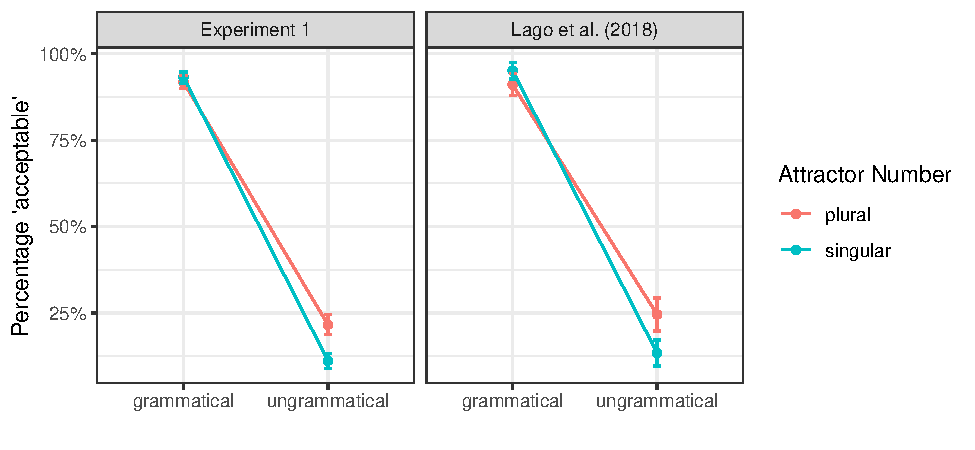
\includegraphics{ongoing_paper_files/figure-latex/exp1AvgResponse-1.pdf}
\caption{\label{fig:exp1AvgResponse}Average response times for experiment 1 and experiment 2.}
\end{figure}

A Bayesian GLM assuming a Bernoulli distribution with a probit-link function was fit to participants' `acceptable' responses. The model's estimates and 95\% credible intervals are shown in Figure \ref{fig:exp1ResponseModel}.

The main effect of \textit{ungrammaticality} (\(\hat{\beta}=-3.09;\) \(CI=[-3.35; -2.84];\) \(P(\beta<0)> .999\)) indicates that, on average, participants were quite good at distinguishing between grammatical and ungrammatical sentences. Meanwhile, the positive interaction between \textit{ungrammaticality} and \textit{attractor number} (\(\hat{\beta}=0.72;\) \(CI=[0.42; 1.02];\) \(P(\beta<0)< .001\)) indicated a larger effect of attractor number in ungrammatical conditions, and thus a number agreement attraction effect.
Importantly, there was no evidence for a three-way interaction between \textit{the presence of ambiguity}, \textit{ungrammaticality} and \textit{attractor number} (\(\hat{\beta}=0.31;\) \(CI=[-0.19; 0.81];\) \(P(\beta<0)= .12\)).

\begin{figure}
\centering
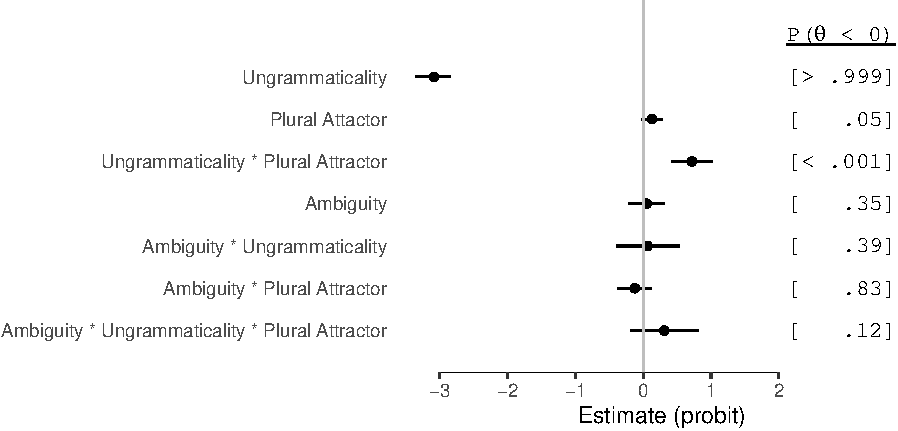
\includegraphics{ongoing_paper_files/figure-latex/exp1ResponseModel-1.pdf}
\caption{\label{fig:exp1ResponseModel}Estimates and 95\% credible intervals for the regression coefficients for the model of Experiment 1 and Lago et al.~(2018).}
\end{figure}

\begin{figure}
\centering
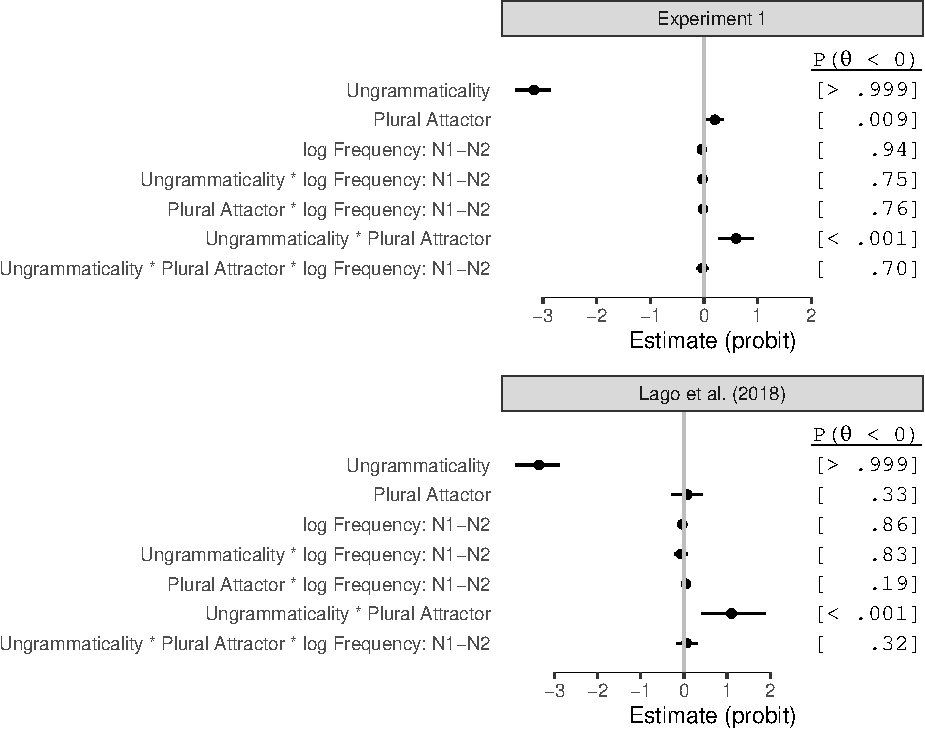
\includegraphics{ongoing_paper_files/figure-latex/exp1ResponseModelSepExp1AndLago-1.pdf}
\caption{\label{fig:exp1ResponseModelSepExp1AndLago}Estimates and 95\% credible intervals for the regression coefficients for Experiment1 and Lago et al.~(2018).}
\end{figure}

\hypertarget{discussion}{%
\subsection{Discussion}\label{discussion}}

In Experiment 1, we have found number attraction effects in Turkish using genitive possessive structures, as it is also attested in Lago et al. (2018). To account for their findings, Lago et al. (2018) assume a cue-based memory retrieval mechanism. That is, they assume that upon reaching the verb, the parser attempts to retrieve its agreement controller (the subject) using a cue-based retrieval mechanism (Lewis \& Vasishth, 2005, p. @JagerEngelmannVasishth:2017). The assumption is that in sentences such as \ref{item:exp1ExperimentalItems}, features such as case and number information are used to identify the agreement controller in memory. In ungrammatical sentences, when the verb bears plural agreement, no NP in memory will match both retrieval cues. However, in ungrammatical plural attractor conditions, the attractor matches one of the cues, which can lead to its erroneous retrieval on some occasions. This cannot happen in ungrammatical singular attractor conditions. This difference in the probability of erroneous retrievals is presumably what surfaced as a number agreement attraction effect, as observed in Lago et al. (2018), and our Experiment 1.

In their work, Lago et al. (2018) argue that the agreement attraction in genitive-possessive structures in Turkish is due to the use of genitive case as a marker of embedded subjects in Turkish, i.e.~differential subject marking (DSM) properties of Turkish (Kornfilt, 2009). They argue that the genitive case in Turkish may not provide strong cue against subjecthood due to DSM while it does in English. Following this logic, we hypothesized that the other phenomenon that gives a strong clue against the subjecthood should inhibit the illusionary dependencies as argued in Nicol et al. (2016). One such phenomenon was present in the experimental items used in Lago et al. (2018): the morpho-phonologic ambiguity between the accusative and the possessive case. Since they use only consonant ending heads, the marking on the head is ambiguous between the accusative and the possessive marking. Following their argumentation, participants may search for other agreement controllers than the possessive marked heads when they are engaged in shallow processing and erroneously assign head as genitive marked distractor.

Nevertheless, we found that when the possessive marker is disambiguated agreement attraction does not diminish in effect size. As seen in Figure \ref{fig:exp1ResponseModel}, we successfully replicated the findings of Lago et al. (2018) with disambiguated head nouns. Thus, we conclude that the morpho-phonological possessive-accusative ambiguity plays no role in number attraction in Turkish.

However, there is an alternative explanation that has yet to be ruled out: task-specific strategies. We hypothesized that readers may engage in an even shallower process in the evaluation of the sentences in which readers decide on the acceptability of the sentence with a faulty state of memory. In our model, we claim that after they read the sentence readers may end up with insufficient information to reliably judge the sentence. Upon such cases, readers may end up using extremely shallow processing methods such as matching the agreement-wise unrelated but form-wise related elements.
We present our hypothesized decision tree in Figure \ref{fig:mptModel}.

\begin{figure}[h]
    \centering
    \tiny\noindent
                      \begin{forest}
                  for tree = {
                  % nodes
                      draw, 
                      align=center,
                      minimum height=5ex,
                      minimum width=3em,
                      font=\linespread{0.84}\selectfont,
                  % tree
                      grow'=0,
                      parent anchor=east,
                      child  anchor=west,
                      s sep = 5mm,    
                      l sep = 10mm, 
                  % edge
                      edge = {semithick},
                  % level styles
                  if level = 0{}{rounded corners=2ex},
                  where n children=0{tier=level, sharp corners}{calign=edge midpoint},
                  % edge labels
                  EL/.style={edge label={node [pos=0.5, fill=white,
                                               font=\scriptsize\sffamily,
                                               inner sep=2pt] {$#1$}}
                                      }
                              }% end for tree
                  [,coordinate
                  [target\\ item,no edge
                      [recolection\\ certainity, EL=r
                          ["yes"]
                      ]
                      [recolection\\ uncertainity, EL=1-r,
                          [guess "yes", tier=L1, EL=g,
                              ["yes"]
                          ]
                          [guess "no", tier=L1, EL=1-g
                              ["no"]
                          ]
                      ]
                  ]
                  [,coordinate, no edge]
                  [target\\ item, no edge
                      [guess "yes", tier=L1, EL=g,
                              ["yes"]
                      ]
                      [guess "no", tier=L1, EL=1-g
                          ["no"]
                      ]
                   ]
                  ]
                      \end{forest} 
    \caption{Proposed multinomial processing tree of how people judge sentences in an agreement attraction task}
    \label{fig:mptModel}
\end{figure}

The aim of our second experiment is to test whether agreement attraction in Turkish is be an instance of a \textit{form-driven processing strategy}. Assuming that readers sometimes engage in shallow processing, they may end up with insufficient information to reliably classify a sentence as (un)acceptable. In such cases, participants may choose to classify sentences with plural-agreement-bearing verbs as acceptable if they have a memory of a nominal plural morpheme in the sentence. Such a response strategy would lead to a larger number of `acceptable' responses in ungrammatical plural attractor conditions than in ungrammatical singular attractor conditions even when there is no interfering noun with plural morphology but, let's say, a plural verb.

\hypertarget{experiment-2}{%
\section{Experiment 2}\label{experiment-2}}

The aim of the Experiment 2 is to control for \emph{form-driven processing strategies} which may be employed by the participants in the processing of Turkish number agreement. A processing mechanism that is driven by form itself, rather than the embedded linguistic features, would predict the comparable agreement attraction effects even when the attractor does not contain a possible nominal plural feature to create interference but contains a form-identical morpheme. To this end, we utilized syncretism between nominal and verbal plural marking in Turkish. Instead of genitive marked nouns, we used the verb of a object relative clauses as in \ref{item:exp2Items}. We expect that under some conditions in which participants do not have sufficient information to rate sentences (un)acceptable, they will decide on the grammaticality of the sentence based on their memory of plural morpheme string, regardless of the feature itself.

\begin{exe}
\ex \label{item:exp2Items}
\gll Tut-tuk-$\emptyset$/lar-(n)ı aşçı mutfak-de sürekli zıpla-dı-$\emptyset$/lar.\\
hire-\Nmlz{}-\Sg{}/\Pl{}-\Poss{} cook kitchen-\Loc{} non-stop jump-\Pst{}-\Sg{}/\Pl{}\\
\glt `The cook that they hired\textsubscript{sg/pl} jumped\textsubscript{sg/pl} in the kitchen non-stop.'
\end{exe}

\emph{Form-driven processing strategies} predicts that we wanted to rule out the possibility of \textit{form-driven processing strategy}, namely participants deciding on the acceptability of a sentence using a memory of plural morpheme in the sentence when they do not have sufficient information to rate sentences (un)acceptable.

\hypertarget{participants-1}{%
\subsection{Participants}\label{participants-1}}

We recruited 79 undergraduate students to participate in Experiment 2 in exchange for course credit. All participants were native speakers of Turkish, with an average age of 21.46 (range: 18 - 31).
Experiment were carried out following the Declaration of Helsinki and the regulations concerning ethics at research in Bo\u{g}azi\c{c}i University. All participants provided informed consent prior to their participation.

\hypertarget{materials-1}{%
\subsection{Materials}\label{materials-1}}

We used 40 sets of sentences like
(\ref{item:exp2ExperimentalItems}), in which we manipulated
(i) the number of the attractor, and
(ii) the number agreement on the verb.
Unlike Experiment 1, we used the verb of a nominalized relative clause (i.e.~\textit{tuttukları}) as an attractor instead of a genitive marked noun.
We took advantage of syncretism between Turkish nominal and verbal plural marker. Both of these morphemes spells-out as \textit{-lAr}, which enables us to check whether agreement attraction in Turkish can be explained by an extremely shallow dependency parsing based on the forms of morphemes rather than linguistic features.

All sentences started with a complex subject NP like \textit{`the cook that they hired'} (\textit{tuttukları aşçı}), in which the verb of the relative clause functioned as the attractor. Because the head noun was singular in all conditions, sentences with plural verb agreement were ungrammatical.\\
We have used the same verbs, and have not changed the distribution of verb types. We also utilized the same or similar adverbials in length.
Relative clauses we used in this experiment are all object relative clauses, and they are all marked with canonical \textit{-dIK} nominalizer. Since Turkish is a pro-drop language, we also dropped the subject within the embedded clause, thus ending up with a one-word object relative clause whose head is the controller of the number agreement on the matrix verb. One example set of experimental items can be seen in \ref{item:exp2ExperimentalItems}.

\begin{exe}
\ex \label{item:exp2ExperimentalItems}
\begin{xlist}

\ex \textsc{Plural Attractor, Ungrammatical (Plural Verb)}\label{item:exp2expitem-plpl}
  \gll *[Tut-tuk-lar-ı \textbf{aşcı}] mutfak-ta sürekli \textbf{zıpla-dı-lar}.\\ 
  hire-\textsc{nmlz}-\textsc{pl}-\textsc{poss}  cook kitchen-\textsc{loc} non-stop  jump-\textsc{pst}-\textsc{pl}.\\
  \glt \textit{`The cook that they hired were jumping in the kitchen non-stop.'}

\ex \textsc{Plural Attractor, Grammatical (Singular Verb)}\label{item:exp2expitem-plsg}
  \gll [Tut-tuk-lar-ı \textbf{aşcı}] mutfak-ta sürekli \textbf{zıpla-dı}.\\ 
  hire-\textsc{nmlz}-\textsc{pl}-\textsc{poss}  cook kitchen-\textsc{loc} non-stop  jump-\textsc{pst}.\\
  \glt \textit{`The cook that they hired was jumping in the kitchen non-stop.'}

\ex \textsc{Singular Attractor, Ungrammatical (Plural Verb)}\label{item:exp2expitem-sgpl}
  \gll *[Tut-tuğ-u \textbf{aşcı}] mutfak-ta sürekli \textbf{zıpla-dı-lar}.\\ 
  hire-\textsc{nmlz}-\textsc{poss}  cook kitchen-\textsc{loc} non-stop  jump-\textsc{pst}-\textsc{pl}.\\
  \glt \textit{`The cook that they hired were jumping in the kitchen non-stop.'}

\ex \textsc{Singular Attractor, Grammatical (Singular Verb)}\label{item:exp2expitem-sgsg}
  \gll [Tut-tuğ-u \textbf{aşcı}] mutfak-ta sürekli \textbf{zıpla-fı}.\\ 
  hire-\textsc{nmlz}-\textsc{poss}  cook kitchen-\textsc{loc} non-stop  jump-\textsc{pst}.\\
  \glt \textit{`The cook that they hired was jumping in the kitchen non-stop.'}
\end{xlist}
\end{exe}

In addition to the experimental items, we used 40 filler sentences of two types, both of which starts with an object relative clause, as illustrated in (\ref{item:exp2FillerItems}). Similar to Experiment 1, our filler items included 20 grammatical sentences with an overtly plural marked verbs, and 20 ungrammatical sentences with no overt plural marking, thus singular.
This was done in order to discourage participants from using a strategy based on verb number.
In all of our filler sentences, the dependency between the first complex NP subject modified with an object relative clause and its verb resolved in an adverbial embedded sentence.
In grammatical fillers, we have used intransitive verbs with a pro-dropped subject as in (\ref{item:exp2FillerItems_plural}).
In ungrammatical fillers, we created the ungrammaticality by placing an adverbial between the bare nominal object and the verb as in (\ref{item:exp2FillerItems_singular}).

\begin{exe}
\ex \label{item:exp2FillerItems}
\begin{xlist}

\ex \label{item:exp2FillerItems_plural} \textsc{Grammatical Filler (Plural Verb)}\\ 
  \gll Oku-t-tuk-lar-ı öğrenci başarılı ol-unca mutlu ol-du-lar.\\ 
  read-\textsc{caus}-\textsc{nmlz}-\textsc{pl}-\textsc{poss}  student successful be-\textsc{nmlz} happy be-\textsc{pst}-\textsc{pl}.\\
  \glt `When the student they sponsored become successful, they became happy.' 

\ex \label{item:exp2FillerItems_singular} \textit{Ungrammatical Filler (Singular Verb)}\\ 
  \gll *Kandır-dığ-ı adam öde-me-yince bulaşık saatlerce yıka-dı.\\ 
  trick-\textsc{nmlz}-\textsc{poss}  man pay-\textsc{neg}-\textsc{nmlz} dish for.hours clean-\textsc{pst}.\\
  \glt Intended:`When the man he tricked did not pay, he cleaned dishes for hours.'
\end{xlist}
\end{exe}

\hypertarget{procedure-1}{%
\subsection{Procedure}\label{procedure-1}}

The experiment was run online, using the web-based platform Ibex Farm (\url{http://spellout.net/ibexfarm/}). For each participant, experiment took approximately 25 minutes to complete.
Participants were asked to provide information regarding their native language and age. They were also asked for their consent to participate in the experiment.
Prior to experimental items, participants read the instructions, and were given 9 practice items with feedback on their accuracy.
Each trial began with a blank screen for 600 ms, followed by a word-by-word RSVP presentantion of the sentence in the center of the screen, followed by an acceptability judgment. Sentences were presented in 30pt font size, and at a rate of 400 ms per word. Between each word, participants saw a blank screen for 100 ms. Participants pressed the key \texttt{P\textquotesingle{}\ for}\textit{acceptable}' and \texttt{Q\textquotesingle{}\ for}\textit{unacceptable}'.
Within instructions, they were told to provide an acceptability rating before 5,000 ms deadline. During the experiment, they were reminded to respondfaster if they did not respond within 5,000 ms.

Participants saw 40 experimental and 40 filler sentences. Experimental sentences were distributed among four different lists according to a Latin-square design. Every participant saw one version of the experiment with a specific list and one item per condition.

\hypertarget{analysis-1}{%
\subsection{Analysis}\label{analysis-1}}

In our analysis, we used the items from Experiment 1, as well as the items from Experiment 2. this decision was made to answer our hypothesis that whether or not participants use the form of the plural suffix rather than the linguistic features. A presence of interaction between the attractor type (\textit{nominal} vs.~\textit{verbal}) and the agreement attraction effect would indicate that people use the linguistic features rather than the form of the plural suffix.

Similar to Experiment 1, we removed the data for all participants who did not exceed the threshold of 25 percentage points in `yes' responses between the grammatical condition and the ungrammatical condition with singular attractors. As a result, we excluded one participant from the Experiment 2, and 10 participant from the Experiment 1.

We used R packages brms (Bürkner, 2018) and rstan (Stan Development Team, 2019) to fit Bayesian hierarchical models (e.g., Gelman \& Hill, 2007). We aalyzed only experimental sentences, and used (i) grammaticality of the sentence, (ii) attractor number, and (iii) type of the plural suffix (i.e., experiment), as well as their interactions as predictors.
Moreover, we used by-participant and by-item intercepts and slopes for all predictors.
Data for Experiment 2, along with our analysis scripts can be found in \url{https://github.com/utkuturk/orc-attractor_numberattraction}.

\hypertarget{results-1}{%
\subsection{Results}\label{results-1}}

\autoref{fig:exp2AvgResponse} shows the average proportions of `acceptable' responses by experimental conditions for Experiment 2.
It shows that ungrammatical sentences with plural attractors are rated as acceptable
(M = 0.05,
SE = 0.01)
as their counterparts with singular attractors
(M = 0.06,
SE = 0.01). The lack of effect (-0.01) compared to the magnitude of the effect in Experiment 1 (-0.01) indicates that the verbal plural morpheme does not trigger an illusionary agreement.
Accuracy rates for grammatical conditions were nearly equal
(M = 0.91 and 0.94,
SE = 0.01 and 0.01, for singular and plural attractors respectively).

\begin{figure}
\centering
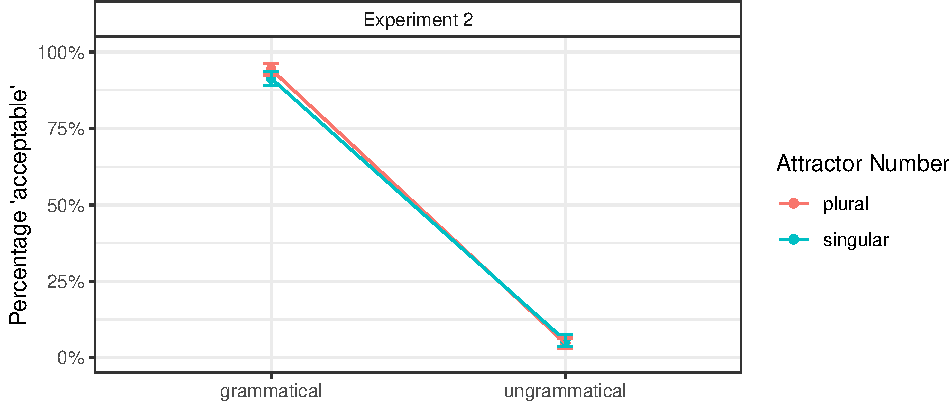
\includegraphics{ongoing_paper_files/figure-latex/exp2AvgResponse-1.pdf}
\caption{\label{fig:exp2AvgResponse}Estimates and 95\% credible intervals for the regression coefficients for Experiment 1 and Experiment 2. Within-subject 95\% confidence intervals in brackets.}
\end{figure}

A Bayesian GLM assuming a Bernoulli distribution with a probit-link function was fit to participants' `acceptable' responses. The model's estimates and 95\% credible intervals are shown in \ref{fig:exp2ResponseModel}.
The main effect of \textit{ungrammaticality} (\(\hat{\beta}=-3.41;\) \(CI=[-3.64; -3.19];\) \(P(\beta<0)> .999\)) indicates that,
on average, participants were quite good at distinguishing between grammatical and ungrammatical sentences.
Meanwhile, there was no evidence for an interaction between \textit{ungrammaticality} and \textit{attractor number} (\(\hat{\beta}=-0.04;\) \(CI=[-0.32; 0.24];\) \(P(\beta<0)= .60\)), indicating
a similar effect of attractor number in ungrammatical conditions compared to grammatical conditions, and thus no number agreement attraction effect.
Importantly, the negative effect between \textit{the presence of the verbal plural}, \textit{ungrammaticality} and \textit{attractor number} (\(\hat{\beta}=-1.08;\) \(CI=[-1.56; -0.61];\) \(P(\beta<0)> .999\)) indicated that the plural morpheme on the verb of the object relative clause lowered the agreement attraction effects.

\begin{verbatim}
## Warning in is.na(x): is.na() (liste veya vekt"or) olmayan 'expression' tipinin
\end{verbatim}

\begin{figure}
\centering
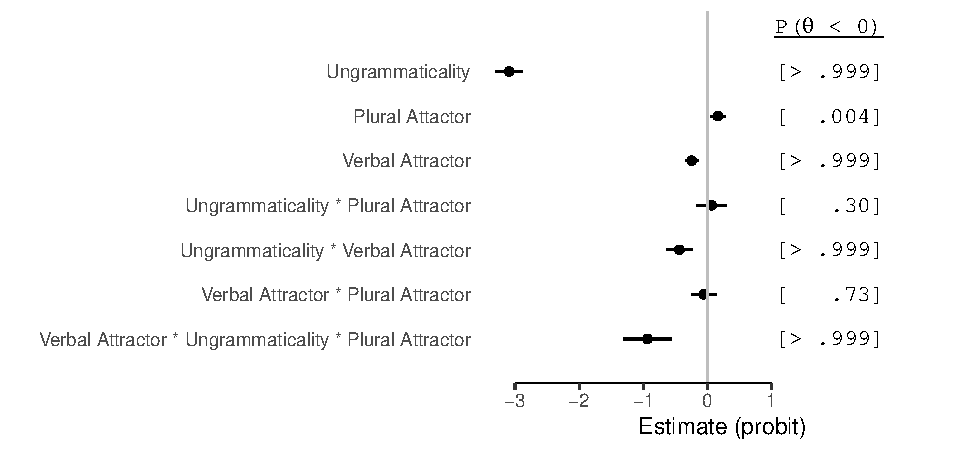
\includegraphics{ongoing_paper_files/figure-latex/exp2ResponseModel-1.pdf}
\caption{\label{fig:exp2ResponseModel}Estimates and 95\% credible intervals for the regression coefficients for a model of Experiment 1 and Experiment 2.}
\end{figure}

\begin{verbatim}
## Warning in is.na(x): is.na() (liste veya vekt"or) olmayan 'expression' tipinin
\end{verbatim}

\begin{figure}
\centering
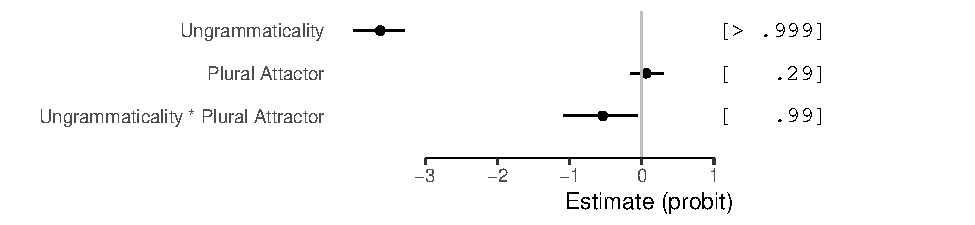
\includegraphics{ongoing_paper_files/figure-latex/exp2ResponseModelExp2Only-1.pdf}
\caption{\label{fig:exp2ResponseModelExp2Only}Estimates and 95\% credible intervals for the regression coefficients for Experiment 2.}
\end{figure}

\hypertarget{discussion-1}{%
\subsection{Discussion}\label{discussion-1}}

In Experiment 2, we could not find any effect of agreement attraction in the acceptability ratings of ungrammatical conditions with a verbal plural attractor. However, number agreement attractions were observed when the attractors were nominal. Even though the forms of the two plural morphemes are the same form-wise, there is a distinct difference between the results of two experiments. One of the indications of zero-effect with verbal plural morpheme is that readers do not make decisions solely based on the form of the elements. This finding contradicts our hypothesized form-driven processing strategy and supports an account of agreement attraction based on the use of abstract linguistic features, rather than mere form.

However, results may be more telling with regards to the other theories of agreement attraction. From the perspective of cue-based retrieval processes, these results tell us that the notion of feature \texttt{+plural} is more complex than previously reported. When a language have syncretic verbal and nominal plurals, it is now reasonable to say that participants distinguish even more and consider the base of the suffixes that they attach. The findings of this experiment indicate towards more fine-grained features needs to be utilized. One other possible explanation within the cue-based retrieval models can be formed around the satisfaction of a dependency. Considering our results, we can manipulate that once a feature is used for a certain representation, it cannot be used again. One can say that the agreement process is completed when the verbal plural on the attractor verb is read. In other words, since the plural morpheme on the attractor verb is not the agreement-triggering morpheme but the probe of the agreement, the retrieval mechanism should not even consider a possibility of retrieving a plural cue from the verb. This may be because either verbal plural are not encoded with \texttt{+plural} cue or they are encoded with \texttt{+plural} and an additional cue which transmits that the dependency is satisfied. This difference would mean that verbal \textit{-lAr} should not start any search for dependency resolution. In contrast to verbal \textit{-lAr}, the plural morpheme on the noun attractor is supposed to be triggering part of the agreement, not the probe.

As for the marking and morphing theories, the results of experiment 2 are completely expected. The effects founds in experiment 2 can be explained by the spreading activation. In the experiment 2 spreading activation were lower due to the distance between the verbal plural and the root note of the head subject compared to the spreading activation with genitive attractors which are closer to root node. Due to the genitive possessor's limited inner complexity and syntactic depth compared to that of relative clause constructions, marking and morphing theories would expect higher contribution from the genitive attractors to the final representation of number information.

\hypertarget{general-discussions}{%
\section{General Discussions}\label{general-discussions}}

We investigated the role of shallow processing in generating agreement attraction effects. We were not able to find any significant finding for the role of morphological local ambiguity (Experiment 1) and the role of form-driven processing strategies (Experiment 2). The results of experiment 1 showed us that the link between the Inhibition Hypothesis and the shallow processing explanation would not predict agreement attraction effects in Turkish. Furthermore, our results of experiment 2 also falsify our hypothesis which was based on the use of morpho-orthographic form for acceptability judgment when there is no enough information.

Our results align with the already existing theories that argue for the role of structural embedding in agreement attraction: MMT. Following the minimalist framework, I assume the following trees as in \ref{syntax:genposs} and \ref{syntax:orc}. Since the plural containing item is embedded deeper in the tree, the verb within the object relative clause would contribute less than the genitive marked NP.

\begin{multicols}{2}

\begin{exe}
\ex \label{syntax:genposs}
\begin{forest}
ned
[DP
  [
    [NP
    [N\\yöneticiler]
    ]
    [D\\-in]
  ]
  [
    [NP\\aşçısı]
    [D]
  ]
]
\path[fill=red] (.parent anchor) circle[radius=2pt];
\path[fill=red] (!1.child anchor) circle[radius=2pt];
\path[fill=red] (!11.child anchor) circle[radius=2pt];
\path[fill=red] (!111.child anchor) circle[radius=2pt];
\end{forest}

\ex \label{syntax:orc}
\begin{forest}
ned
[DP
  [
    [
      [pro]
      [
        [VP
          [NP\\ t\textsubscript{1}]
          [V\\Tuttukları]
        ]
        [T]
      ]
    ]
    [C]
  ]
  [
    [NP\\aşçı]
    [D]
  ]
]
\path[fill=red] (.parent anchor) circle[radius=2pt];
\path[fill=red] (!1.child anchor) circle[radius=2pt];
\path[fill=red] (!11.child anchor) circle[radius=2pt];
\path[fill=red] (!112.child anchor) circle[radius=2pt];
\path[fill=red] (!1121.south) circle[radius=2pt];
\path[fill=red] (!11212.child anchor) circle[radius=2pt];
\end{forest}
\end{exe}

\end{multicols}

Additionally, our results suggest fine-tuning within the cue-based retrieval explanation. Retrieving \texttt{+plural} is not enough as shown in our experiment 2. Other pieces of information are necessary to stimulate agreement attraction effects. One possibility is retrieval only happens among the non-satisfied dependencies. Another possibility is that the base of the plural is also encoded.

As for our hypothesized shallow processing explanation for agreement attraction, we could not provide any evidence towards it. We can say that with these structures we were not able to generate agreement attractions.

\hypertarget{conclusion}{%
\section{Conclusion}\label{conclusion}}

In this paper, we reported two experiments on number agreement attraction effects in Turkish. We observed number agreement attraction with nominal plural morphemes in experiment 1, but not with verbal plural morphemes in experiment 2. In Experiment 1, our findings were parallel to those of Lago et al. (2018) with unambiguously possessive marked heads. In Experiment 2, we failed to observe number agreement attraction effects with object relative clause attractors.

Our results suggest that morpho-phonological ambiguities do not play a role in number agreement attraction in Turkish, and speakers do not use form solely in decision making processes. These findings support an agreement attraction theory which makes use of abstract linguistic features.

\hypertarget{references}{%
\section{References}\label{references}}

\begingroup
\setlength{\parindent}{-0.5in}

\hypertarget{refs}{}
\begin{cslreferences}
\leavevmode\hypertarget{ref-AvetisyanEtAl:2020}{}%
Avetisyan, S., Lago, S., \& Vasishth, S. (2020). Does case marking affect agreement attraction in comprehension? \emph{Journal of Memory and Language}, \emph{112}, 104087.

\leavevmode\hypertarget{ref-BadeckerKuminiak:2007}{}%
Badecker, W., \& Kuminiak, F. (2007). Morphology, agreement and working memory retrieval in sentence production: Evidence from gender and case in Slovak. \emph{Journal of Memory and Language}, \emph{56}(1), 65--85.

\leavevmode\hypertarget{ref-BergenGibson:2012}{}%
Bergen, L., \& Gibson, E. (2012). Agreement errors as rational encoding errors. In \emph{Poster presented at the 25th annual cuny conference on human sentence processing, new york, ny}.

\leavevmode\hypertarget{ref-BockEberhard:1993}{}%
Bock, K., \& Eberhard, K. M. (1993). Meaning, sound and syntax in english number agreement. \emph{Language and Cognitive Processes}, \emph{8}(1), 57--99. \url{https://doi.org/10.1080/01690969308406949}

\leavevmode\hypertarget{ref-Bock1991}{}%
Bock, K., \& Miller, C. A. (1991). Broken agreement. \emph{Cognitive Psychology}, \emph{23}(1), 45--93.

\leavevmode\hypertarget{ref-brms}{}%
Bürkner, P.-C. (2018). \emph{Advanced Bayesian multilevel modeling with the R package brms}. \emph{The R Journal} (Vol. 10, pp. 395--411). \url{https://doi.org/10.32614/RJ-2018-017}

\leavevmode\hypertarget{ref-Dillon2013a}{}%
Dillon, B., Clifton, C., \& Frazier, L. (2013). Pushed aside: Parentheticals, memory and processing. \emph{Language, Cognition and Neuroscience}, \emph{29}(4), 483--498. \url{https://doi.org/10.1080/01690965.2013.866684}

\leavevmode\hypertarget{ref-Eberhard:1997}{}%
Eberhard, K. M. (1997). The marked effect of number on subject--verb agreement. \emph{Journal of Memory and Language}, \emph{36}(2), 147--164.

\leavevmode\hypertarget{ref-EberhardEtAl:2005}{}%
Eberhard, K. M., Cutting, J. C., \& Bock, K. (2005). Making syntax of sense: Number agreement in sentence production. \emph{Psychological Review}, \emph{112}(3), 531.

\leavevmode\hypertarget{ref-FerreiraBaileyFerraro:2002}{}%
Ferreira, F., Bailey, K. G. D., \& Ferraro, V. (2002). Good-Enough Representations in Language Comprehension. \emph{Current Directions in Psychological Science}, \emph{11}(1).

\leavevmode\hypertarget{ref-FranckColonnaRizzi:2015}{}%
Franck, J., Colonna, S., \& Rizzi, L. (2015). Task-dependency and structure-dependency in number interference effects in sentence comprehension. \emph{Frontiers in Psychology}, \emph{6}(MAR), 1--15. \url{https://doi.org/10.3389/fpsyg.2015.00349}

\leavevmode\hypertarget{ref-FranckEtAl:2002}{}%
Franck, J., Vigliocco, G., \& Nicol, J. (2002). Subject-verb agreement errors in french and english: The role of syntactic hierarchy. \emph{Language and Cognitive Processes}, \emph{17}(4), 371--404.

\leavevmode\hypertarget{ref-GelmanHill2007}{}%
Gelman, A., \& Hill, J. (2007). \emph{Data Analysis Using Regression and Multilevel/Hierarchical Models}. Cambridge, UK: Cambridge University Press.

\leavevmode\hypertarget{ref-GibsonThomas:1999}{}%
Gibson, E., \& Thomas, J. (1999). Memory Limitations and Structural Forgetting: The Perception of Complex Ungrammatical Sentences as Grammatical. \emph{Language and Cognitive Processes}, \emph{14}(3).

\leavevmode\hypertarget{ref-HammerlyEtAl:2019}{}%
Hammerly, C., Staub, A., \& Dillon, B. (2019). The grammaticality asymmetry in agreement attraction reflects response bias: Experimental and modeling evidence. \emph{Cognitive Psychology}, \emph{110}, 70--104.

\leavevmode\hypertarget{ref-Haussler2009}{}%
Häussler, J., \& Bader, M. (2009). Agreement checking and number attraction in sentence comprehension: Insights from german relative clauses. \emph{Trav. Cercle Linguist. Prague}, \emph{7}.

\leavevmode\hypertarget{ref-JagerEngelmannVasishth:2017}{}%
Jäger, L. A., Engelmann, F., \& Vasishth, S. (2017). Similarity-based interference in sentence comprehension: Literature review and Bayesian meta-analysis. \emph{Journal of Memory and Language}, \emph{94}, 316--339. \url{https://doi.org/10.1016/j.jml.2017.01.004}

\leavevmode\hypertarget{ref-kornfilt2009dom}{}%
Kornfilt, J. (2009). DOM and two types of dsm in turkish. In \emph{Differential subject marking} (pp. 79--111). Springer.

\leavevmode\hypertarget{ref-LagoEtAl2018}{}%
Lago, S., Felser, C., Gračanin-Yuksek, M., Demir, O., Kırkıcı, B., \& Şafak, D. F. (2018). Straight from the horse's mouth: Agreement attraction effects with Turkish possessors. \emph{Linguistic Approaches to Bilingualism}, \emph{12}(1), 1--29. \url{https://doi.org/10.1075/lab.17019.lag}

\leavevmode\hypertarget{ref-LagoEtAl:2015}{}%
Lago, S., Shalom, D. E., Sigman, M., Lau, E. F., \& Phillips, C. (2015). Agreement attraction in Spanish comprehension. \emph{Journal of Memory and Language}, \emph{82}, 133--149. \url{https://doi.org/10.1016/j.jml.2015.02.002}

\leavevmode\hypertarget{ref-Levy2008}{}%
Levy, R. (2008). Expectation-based syntactic comprehension. \emph{Cognition}, \emph{106}(3), 1126--1177. \url{https://doi.org/10.1016/j.cognition.2007.05.006}

\leavevmode\hypertarget{ref-LewisVasishth2005}{}%
Lewis, R. L., \& Vasishth, S. (2005). An activation-based model of sentence processing as skilled memory retrieval. \emph{Cognitive Science}, \emph{29}(3), 375--419. \url{https://doi.org/10.1207/s15516709cog0000_25}

\leavevmode\hypertarget{ref-NicenboimEtAl:2018}{}%
Nicenboim, B., Vasishth, S., Engelmann, F., \& Suckow, K. (2018). Exploratory and confirmatory analyses in sentence processing: A case study of number interference in german. \emph{Cognitive Science}, \emph{42}, 1075--1100.

\leavevmode\hypertarget{ref-NicolEtAl:2016}{}%
Nicol, J. L., Barss, A., \& Barker, J. E. (2016). Minimal interference from possessor phrases in the production of subject-verb agreement. \emph{Frontiers in Psychology}, \emph{7}, 548.

\leavevmode\hypertarget{ref-Nicoletal:1997}{}%
Nicol, J. L., Forster, K. I., \& Veres, C. (1997). Subject--verb agreement processes in comprehension. \emph{Journal of Memory and Language}, \emph{36}(4), 569--587.

\leavevmode\hypertarget{ref-OteroKintsch:1992}{}%
Otero, J., \& Kintsch, W. (1992). Failures to detect contradictions in a text: What readers believe versus what they read. \emph{Psychological Science}, \emph{3}(4), 229--236.

\leavevmode\hypertarget{ref-ParkerEtAl:2015}{}%
Parker, D., Lago, S., \& Phillips, C. (2015). Interference in the processing of adjunct control. \emph{Frontiers in Psychology}, \emph{6}(September), 1--13. \url{https://doi.org/10.3389/fpsyg.2015.01346}

\leavevmode\hypertarget{ref-PaspaliMarinis:2020}{}%
Paspali, A., \& Marinis, T. (2020). Gender agreement attraction in greek comprehension. \emph{Frontiers in Psychology}, \emph{11}, 717.

\leavevmode\hypertarget{ref-PatsonHusband:2016}{}%
Patson, N. D., \& Husband, E. M. (2016). Misinterpretations in agreement and agreement attraction. \emph{The Quarterly Journal of Experimental Psychology}, \emph{69}(5), 950--971.

\leavevmode\hypertarget{ref-PearlmutterGarnseyBock:1999}{}%
Pearlmutter, N. J., Garnsey, S. M., \& Bock, K. (1999). Agreement Processes in Sentence Comprehension. \emph{Journal of Memory and Language}, \emph{41}.

\leavevmode\hypertarget{ref-PhillipsEtAl:2011}{}%
Phillips, C., Wagers, M., \& Lau, E. F. (2011). Grammatical Illusions and Selective Fallibility in Real-Time Language Comprehension. \emph{Syntax and Semantics 37: Experiments at the Interfaces}, \emph{37}(2011), 53--186.

\leavevmode\hypertarget{ref-ReifegersteEtAl:2016}{}%
Reifegerste, J., Hauer, F., \& Felser, C. (2016). Agreement processing and attraction errors in aging: evidence from subject-verb agreement in German. \emph{Aging, Neuropsychology, and Cognition}, \emph{00}(00), 1--31. \url{https://doi.org/10.1080/13825585.2016.1251550}

\leavevmode\hypertarget{ref-Slioussar:2016}{}%
Slioussar, N., \& Malko, A. (2016). Gender agreement attraction in russian: Production and comprehension evidence. \emph{Frontiers in Psychology}, \emph{7}, 1651.

\leavevmode\hypertarget{ref-stan}{}%
Stan Development Team. (2019). RStan: The R interface to Stan. Retrieved from \url{http://mc-stan.org/}

\leavevmode\hypertarget{ref-TannerEtAl:2014}{}%
Tanner, D., Nicol, J., \& Brehm, L. (2014). The time-course of feature interference in agreement comprehension: Multiple mechanisms and asymmetrical attraction. \emph{Journal of Memory and Language}, \emph{76}, 195--215.

\leavevmode\hypertarget{ref-TuckerEtAl:2015}{}%
Tucker, M. A., Idrissi, A., \& Almeida, D. (2015). Representing number in the real-time processing of agreement: Self-paced reading evidence from Arabic. \emph{Frontiers in Psychology}, \emph{6}(MAR), 1--21. \url{https://doi.org/10.3389/fpsyg.2015.00347}

\leavevmode\hypertarget{ref-ViglioccoEtAl:1995}{}%
Vigliocco, G., Butterworth, B., \& Semenza, C. (1995). Constructing subject-verb agreement in speech: The role of semantic and morphological factors. \emph{Journal of Memory and Language}, \emph{34}(2), 186--215.

\leavevmode\hypertarget{ref-WagersEtAl:2009}{}%
Wagers, M. W., Lau, E. F., \& Phillips, C. (2009). Agreement attraction in comprehension: Representations and processes. \emph{Journal of Memory and Language}, \emph{61}(2), 206--237. \url{https://doi.org/10.1016/j.jml.2009.04.002}
\end{cslreferences}

\endgroup


\end{document}
